\documentclass[french]{article}
\usepackage{graphicx}
\usepackage{babel}
\usepackage[a4paper, total={6in, 10in}]{geometry}
\usepackage{graphicx}
\usepackage{listings}
\usepackage{color}
\usepackage{pdfpages}

\usepackage[svgnames]{xcolor} % Required for colour specification
\usepackage[utf8]{inputenc} % Required for inputting international characters
\usepackage[T1]{fontenc} % Output font encoding for international characters
\usepackage{fouriernc} % Use the New Century Schoolbook font

\DeclareGraphicsExtensions{.pdf,.png,.jpg}
% listings color configuration to display beautifuuul code
\definecolor{Monokaigreen}{rgb}{0.42,0.72,0.18}
\definecolor{Monokaimagenta}{rgb}{0.86,0.08,0.24}
\definecolor{Monokaiblue}{rgb}{0.40,0.85,0.94}
\definecolor{Monokaibg}{rgb}{0.15,0.16,0.13}
\definecolor{splashedwhite}{rgb}{1.0, 0.99, 1.0}
\definecolor{richelectricblue}{rgb}{0.03, 0.57, 0.82}
\definecolor{pinegreen}{rgb}{0.0, 0.47, 0.44}
\definecolor{ivory}{rgb}{1.0, 1.0, 0.94}
\definecolor{ghostwhite}{rgb}{0.97, 0.97, 1.0}
\definecolor{floralwhite}{rgb}{1.0, 0.98, 0.94}
\definecolor{gray}{rgb}{0.5,0.5,0.5}


\lstset{frame=shadowbox,
	language=Java,
	aboveskip=3mm,
	belowskip=3mm,
	showstringspaces=false,
	columns=flexible,
	basicstyle={\small\ttfamily},
	numbers=left,
	numberstyle=\tiny\color{gray},
	keywordstyle=\color{Monokaibg}\bfseries,
	commentstyle=\color{pinegreen},
	stringstyle=\color{Monokaigreen},
	breaklines=true,
	breakatwhitespace=false,
	tabsize=3,
	captionpos=b,                    % sets the caption-position to bottom
	frame=single,
	rulecolor=\color{gray},
}

\title{Sections and Chapitres}
\author{Quentin Gigon}
\date{ }

\begin{document}

\begin{titlepage} % Suppresses headers and footers on the title page
	
	\centering % Centre everything on the title page
	
	%------------------------------------------------
	%	Top rules
	%------------------------------------------------
	
	\rule{\textwidth}{1pt} % Thick horizontal rule
	
	\vspace{2pt}\vspace{-\baselineskip} % Whitespace between rules
	
	\rule{\textwidth}{0.4pt} % Thin horizontal rule
	
	\vspace{0.1\textheight} % Whitespace between the top rules and title
	
	%------------------------------------------------
	%	Title
	%------------------------------------------------
	
	\textcolor{Red}{ % Red font color
		{\Huge TB}\\[0.5\baselineskip] % Title line 1
	}
	
	\vspace{0.025\textheight} % Whitespace between the title and short horizontal rule
	
	\rule{0.3\textwidth}{0.4pt} % Short horizontal rule under the title
	
	\vspace{0.1\textheight} % Whitespace between the thin horizontal rule and the author name
	
	%------------------------------------------------
	%	Author
	%------------------------------------------------
	
	{\Large \textsc{Quentin Gigon}} % Author name
	
	\vfill % Whitespace between the author name and publisher
	
	%------------------------------------------------
	%	Publisher
	%------------------------------------------------
	
	{\large\textsc{HEIG-VD}} % Publisher
	
	\vspace{0.1\textheight} % Whitespace under the publisher text
	
	%------------------------------------------------
	%	Bottom rules
	%------------------------------------------------
	
	\rule{\textwidth}{0.4pt} % Thin horizontal rule
	
	\vspace{2pt}\vspace{-\baselineskip} % Whitespace between rules
	
	\rule{\textwidth}{1pt} % Thick horizontal rule
	
\end{titlepage}

\maketitle

\tableofcontents
\newpage

\section{Introduction au projet}
Le but de ce travail est de pouvoir visualiser et gérer l'affichage de divers flux d'information sur les écrans des différents campus de la HEIG, comme par exemple les horaires de cours, les news de la RTS, les réservations de salles, etc, à travers une interface web.

\section{Cahier des charges}
A remettre à jour!!

\subsection{Contraintes et besoins}
Les besoins principaux de cette application sont les suivants:
\begin{itemize}
	\item Gestion de l'affichage de flux d'information sur des écrans dans la HEIG-VD (smartTV ou ordinateur) par une interface web.
	\item Protocole concis de communication entre les écrans et le serveur limitant les échanges.
	\item Affichage de flux "controlés" (générés par l'application, par exemple un flux RSS) et "non-controlés" (flux de la RTS, horaires des cours, etc).
	\item Un Schedule qui s'occupe de changer les flux affichés selon un horaire prédéfini.
	\item Une modélisation générique des flux et une factorisation de ceux venant de sources externes afin de pouvoir les envoyer de la même manière aux écrans
	\item La possibilité de diffuser plusieurs types de médias (images, vidéos, etc)
	\item La possibilité de passer outre le Schedule et d'afficher un flux voulu (annonce importante, etc) avec reprise de l'exécution prévue par la suite. \newline
\end{itemize}


\textbf{Quelques précisions:}
Un Schedule est un "horaire" qui gère le changement de flux selon un ordre choisi par l'utilisateur. Il n'y aura pas qu'un seul Schedule mais plutôt la possibilité d'en créer plusieurs qui soient assignables à un écran ou groupe d'écrans.
\newline


Les contraintes principales quand à elles sont les suivantes:
\begin{itemize}
	\item L'affichage des flux doit être fait dans un navigateur supportant le Javascript, HTLM5 et CSS3.
	\item Il doit y avoir une base de données qui enregistre les utilisateurs ainsi que les écrans.
	\item Il y a plusieurs types d'utilisateurs qui, selon leur emplacement (campus) et/ou leur niveau d'autorisation, peuvent modifier l'affichage des écrans.
	\item Le système doit être tolérant face aux panne, avec une reprise automatique.
	\item Le système doit disposer d'une interface simple et être utilisable par des gens du domaine et par des personnes non-initiées.
\end{itemize}


\subsection{Fonctionnalités}
Les fonctionnalités nécessaires et principales du programme sont divisées en plusieurs catégories:
\begin{itemize}
	\item \textbf{Frontend}
	\begin{enumerate}
		\item Interface de login et register sur le site (register dans le cadre du TB)
		\item Ecrans
		\begin{enumerate}
			\item Visualisation des écrans actifs et de leur emplacement sur le campus (une "carte" par site)
			\item Visualisation des informations d'un écran spécifique (et groupe d'écrans)
			\item Modification de la diffusion actuelle sur un écran/groupe d'écrans (flux "hors-schedule", attribution à un Schedule, arrêt de la diffusion, ...)
		\end{enumerate}
		\item Flux
		\begin{enumerate}
			\item Opérations CRUD sur les flux (interface de création)
			\item Visualisation des flux utilisables par le système et infos sur leur contenu
		\end{enumerate}
		\item Schedules
		\begin{enumerate}
			\item Opérations CRUD sur les Schedules (interface de création)
			\item Visualisation des Schedules utilisables par le système et infos sur leur contenu et horaire
		\end{enumerate}
		\end{enumerate}
	\item \textbf{Backend - Play!}
	\begin{enumerate}
		\item Ecrans
		\begin{enumerate}
			\item Opérations CRUD sur les écrans
			\item Emission de token d'authentification pour la connexion des écrans
		\end{enumerate}
		\item Flux
		\begin{enumerate}
			\item Opérations CRUD sur les flux
			\item Diffusion de flux aux écrans selon un Schedule
			\item Diffusion de flux hors-schedule (annonces, alertes, etc)
			\item Formatage et mise en page des flux externes (RTS ou autre)
		\end{enumerate}
		\item Schedules
		\begin{enumerate}
			\item Opérations CRUD sur les Schedules
			\item Assignation d'un Schedule à un écran/groupe d'écrans
		\end{enumerate}
		\item Utilisateurs
		 \begin{enumerate}
			\item Register 
			\item Login 
			\item Niveaux d'autorisation
		\end{enumerate}
	\end{enumerate}
	
	\item \textbf{Base de données}
	\begin{enumerate}
		\item Utilisateurs avec différents niveaux d'autorisations
		\item Ecrans, avec leurs caractéristiques et emplacement
		\item Flux utilisés par le système
		\item Schedules de flux \newline
	\end{enumerate}
\end{itemize}

Les fonctionnalités suivantes sont considérées comme secondaires et seront réalisées si le temps le permet:
\begin{itemize}
	\item \textbf{Frontend}
	\begin{enumerate}
		\item Modification en live du contenu d'un flux
	\end{enumerate}
	\item \textbf{Backend}
	\begin{enumerate}
		\item Monitoring de l'état des écrans (log du dernier échange avec l'écran)
		\item Schedul-ception (Schedule dans un Schedule)
	\end{enumerate}
\end{itemize}

\subsection{Echéancier}

Le travail sera divisé en 4 parties :
\begin{itemize}
	\item \textbf{Analyse et Modélisation} (2 semaines) \newline
	Analyse des contraintes et besoins du travail et modélisation d'un système parvenant à y répondre (schémas de DB, modélisation des flux, etc)
	\item \textbf{Architecture} (1 semaine) \newline
	Création d'une architecture de code permettant la réalisation d'un programme efficace, modulable et améliorable par la suite
	\item \textbf{Développement et Tests} (7 semaines) \newline
	Codage de l'application, en commençant par le serveur et en finissant avec le frontend.  
	Création de la base de données en parallèle.
	Tests unitaires et fonctionnels (60-70\% de coverage visé)
	\item \textbf{Rapport et Documentation} (3 semaines) \newline
	\end{itemize}
	
Total: env. 13 semaines à partir du 25.02 \newpage

\section{Mockups}


\section{Présentation des technologies utilisées}

\subsection{Framework Play!}
Play! est un framework web open-source qui suit le modèle MVC et qui permet d'écrire rapidement des application web en Java (ou en Scala). A la différence d'autre frameworks Java, Play! est \textit{stateless}, ce qui veut dire qu'il n'y a pas de session JavaEE créée à chaque connexion. 
Il fourni aussi à ses utilisateurs des frameworks de tests unitaires et fonctionnels, à savoir JUnit et Selenium.


\subsection{EventSource}
Les EventSource, ou Server-Sent Events (SSE), sont une technologie permettant à un navigateur internet de recevoir des mises à jour automatiques d'un serveur par une connexion HTTP persistante. L'API Javascript (\textit{Server-Sent Events EventSource API}) fut instaurée la première fois dans Opera en 2006 et a été normalisée dans le cadre de HTML5. \par
Les Events envoyés sont au format \textit{text/event-stream} et sont reçus par le navigateur sous la forme d'Event de type \textit{message} La connexion reste ouverte tant qu'elle n'a pas été fermée par le navigateur, et contrairement aux WebSockets, les SSE sont uni-directionnels et ne permettent donc pas aux clients de communiquer avec le serveur. 

\subsection{PostgreSQL}
PostgreSQL est un système de gestion de base de données relationnelle et open-source. La différence principale entre PostgreSQL et ses concurrents est la prise en charge de plus de types de donnée que les types traditionnels (entiers, caractères, ...).

\subsection{JPA}
La Java Persistence API (JPA) est une interface de programmation permettant aux utilisateurs de la plateforme Java (SE et EE) d'organiser facilement et clairement leurs données relationnelles. Elle utilise des annotations pour définir des "objet-métiers" qui serviront d'interface entre la base de données et l'application. \newline
JPA définit aussi le Java Persistence Query Language (JPQL), qui est utilisé pour créer les requêtes SQL dans le cadre de JPA. Les requêtes effectuées dans ce langage ressemblent beaucoup à du SQL classique, sauf que le JPQL fonctionne avec des entités (créées avec des annotations) plutôt que des tables de la base de données.

\subsection{JWT}
Un JSON Web Token est un standard ouvert permettant l'échange sécurisé de jetons d'accès entre plusieurs parties. Les jetons sont signés à l'aide d'une clé privée (très souvent le serveur) et fournis aux client qui doivent l'intégrer à leurs prochaines requêtes. Un jeton n'est pas associé à un utilisateur mais plutôt à un rôle (p.ex. administrateur) et à une durée de validité définie par le serveur également. Ils sont très souvent utilisés pour gérer des utilisateurs (login).

\subsection{HTML5}
HTML5 est la dernière version majeure du HTML (octobre 2014). Elle vient avec plein de nouveaux élément, comme la balise \textit{video}, qui permet d'insérer un contenu vidéo en streaming dans un fichier HTML, ou encore \textit{footer}, qui lui permet de facilement afficher du texte en bas de page.

\section{Réalisation technique}

\subsection{Controllers}

\subsubsection{EventSource Java}

\subsection{Views}

\subsubsection{EventSource Javascript}

\newpage
\section{Analyse et Architecture}

\subsection{Team et site}

\subsubsection{Site}
Un site représente un emplacement physique de l'HEIG-VD, donc les sites de Cheseaux, St-Roch et Y-Park (pour l'instant en tout cas). Ils servent principalement à localiser les écrans et restreindre les flux. 

\subsubsection{Team}
Les Teams ont une importance fondamentale dans l'architecture du programme. En effet, une Team n'a accès qu'aux éléments nécessaire pour elle, donc un nombre limité d'écrans (et groupes d'écrans), de Schedules et de Diffuser. Une Team est composée d'un admin (TeamAdmin) et de simples membres. L'admin est le seul à pouvoir créer des Schedules.

\subsection{Organisation des flux}

\subsubsection{Flux}
Un flux dans ce programme représente un contenu à afficher envoyé aux écrans. Ils se divisent en trois catégories principales:
\begin{itemize}
	\item Des flux externes (flux de la RTS)
	\item Des flux gérés par l'application (flux RSS)
	\item Des flux internes, avec la possibilité de les interroger pour savoir s'ils ont du contenu à afficher (réservation de salle, élection du CoRe) 
\end{itemize}
Chaque flux est caractérisé par au moins une URL, une durée d'affichage minimum, un nom et un type. Le type d'un flux détermine la manière dont il va être traité par l'application et affiché par les écrans. Par exemple: video, image, texte, "normal".\newline
De plus, il y a deux sorte de flux: des flux généraux et des flux localisés (LocatedFlux). Un flux localisé est uniquement affichable sur le Site correspondant. Cela afin de pouvoir p.ex. créer un seul flux pour les horaires, qui selon le site ou il est envoyé prend un paramètre de requête différent (-> http://heig.com/horaires?site=che). Cette information sera stockée dans la base de donnée. \newline
Et enfin un flux peut être un flux marketing (un Boolean dans le modèle). Cette information est utilisée pour créer des groupes de flux marketing dans lesquels le serveur peut piocher pour remplacer des flux actifs mais sans information utile pour le moment. Ce système permet donc d'avoir des flux de "fallback" à afficher, qu'ils soit généraux ou localisés. \newline \par
Pour revenir aux flux gérés par l'application (flux RSS), un template d'affichage générique sera fourni avec l'application afin de pouvoir facilement ajouter de nouveaux flux. Les informations seront récupérées à intervalles réguliers par le serveur afin de garder les flux à jour.

\subsubsection{Schedules}
Un Schedule représente un horaire de flux, c'est-à-dire une liste de flux, chacun associé à une heure de démarrage. Un Schedule n'est pas assigné à des écrans à sa création mais au moment de son activation pour permettre  une réutilisation plus facile des Schedules créés. Chaque chef d'équipe peut en créer qui seront utilisables par tous les membres de son équipe (modifiable par eux potentiellement ?). Ils sont utilisés pour des flux de type "régulier", donc pas des messages uniques ou promotionnels. \newline
Un Schedule activé devient un RunningSchedule, une entité temporaire qui existe uniquement tant que le Schedule reste actif. C'est cette entité-ci qui est reliée à des écrans. Et donc chaque fois qu'un flux doit être démarré, le RunningSchedule donne l'ordre d'envoyer un nouvel Event aux écrans concernés (voir section Affichage). 

\subsubsection{Diffuser}
Un Diffuser est quand à lui utilisé pour diffuser un flux de catégorie marketing ou un message unique sur une quantité X d'écrans. Ils fonctionnent en changeant les Schedules actifs associés à ces écrans pour ajouter le flux souhaité dans leur horaire. Ce système offre plusieurs possibilités de customisation, comme spécifier la durée du flux ou limiter dans le temps la diffusion de ce flux (p.ex. modifier les Schedules actifs seulement pendant une semaine et revenir à l'état de base après). Au moment de l'ajout du flux dans le Schedule, des vérifications sont faites pour garantir un bon fonctionnement par la suite (on peut imaginer que l'heure choisie pour le nouveau flux soit déjà prise, il faudra alors avertir l'utilisateur qu'il ne peut effectuer cette action ou alors autoriser l'action mais adapter l'heure de démarrage du nouveau flux pour ce Schedule). \newline
Comme pour les Schedules, un Diffuser actif est un RunningDiffuser, lui aussi une entité temporaire qui reste active selon la validité spécifiée à sa création. Un fois que le RunningDiffuser est arrivé en fin de vie, le flux qu'il avait rajouté dans les RunningSchedules est enlevé.


\subsection{Ecrans}

\subsubsection{Affichage}
Pour afficher les flux sur les écrans, les technologies autorisées sont le HTML5, CSS3 et Javascript pur (sans frameworks). On peut très facilement afficher dans un navigateur (Chrome en l'occurence) le contenu associé à une URL grâce aux iframes (insert doc here ?), donc il fallait un moyen pour les écrans de recevoir une URL à afficher. Les EventSource sont une solution tout à fait adaptée pour ce programme, car ils évitent aux écrans de faire des requêtes au serveur pour recevoir leur flux.

\subsubsection{Events}
Un des problèmes à résoudre était : Comment envoyer les bons Event aux bons écrans ? Il y avait deux manières principales de faire, soit envoyer tous les Events à tous les écrans avec la liste des écrans concernés, soit générer dynamiquement des endpoints pour chaque Schedule. Pour des raisons de simplicité et parce que le nombre d'écrans restera raisonnable, la première possibilité a été choisie. \newline
Les Events générés par les Schedules sont donc envoyés à tous les écrans s'étant connecté auprès du serveur. Chaque Event contient les adresses MAC des écrans concernés et c'est à l'écran de vérifier s'il est concerné par l'Event qu'il vient de recevoir. Pour se faire, il récupère son adresse MAC dans les cookies (ajouté par le serveur pendant la phase d'authentification) et la compare avec celles reçues. 

\subsubsection{Authentification}
Un écran ne peut recevoir d'Event qu'une fois authentifié. Leur authentification se fait donc à l'aide de leur adresse MAC, car il y a le projet plus tard d'incorporer le WakeOnLan (qui utilise donc les adresses MAC) pour avoir un meilleur contrôle sur les écrans. \newline
L'accès des écrans au Flux Manager (donc le serveur) se fait en deux étapes. Il faut d'abord que l'écran se connecte à la route d'authentification des écrans, tout en spécifiant comme paramètre de requête son adresse MAC (p.ex. http://server/screens/auth?mac=1234). Là, si l'adresse est inconnue par le serveur, il nous renvoie un code permettant l'ajout de l'écran dans le système depuis le site web. Si l'adresse est connue, il ajoute un nouveau cookie contenant l'adresse MAC de l'écran, passe l'écran comme actif et le redirige vers le Flux Manager.

\subsubsection{Groupe d'écrans}
Les groupes d'écrans sont créés par des chefs d'équipe et donc uniquement disponible à l'intérieur d'une Team (on pourrait aussi imaginer des groupes communs à toutes les Teams). Ils servent à regrouper les écrans selon leur utilité, pour faciliter leur assignement à un Schedule. Par exemple, un groupe d'écran possible serait celui des écrans du hall de Cheseaux. \newline
Un écran peut faire partie de plusieurs groupes, mais comme précisé plus haut, il ne peut être associé qu'a un RunningSchedule à la fois. Il y aura donc des vérifications qui seront faites au moment d'activer un Schedule sur un groupe d'écran pour empêcher ceci.

\newpage

		
\section{Protocole de communication écran-serveur}
TODO: refaire les images.\newline
	Le protocole ci-dessous explique et détaille la communication entre les écrans et le serveur, ainsi que les erreurs potentielles et leur prise en charge. 
	
\subsection{Ecran inconnu du serveur}
	Dans ce cas de figure, l'écran n'a pas encore été ajouté au système par l'administrateur, et donc le serveur ne reconnait pas son adresse MAC lors de la connexion. A ce moment, il lui renvoie une page HTML qui affiche un code (propre à chaque écran) a utiliser pour introduire l'écran dans le système.
	
		\begin{figure}[hbt!]
			\centering
			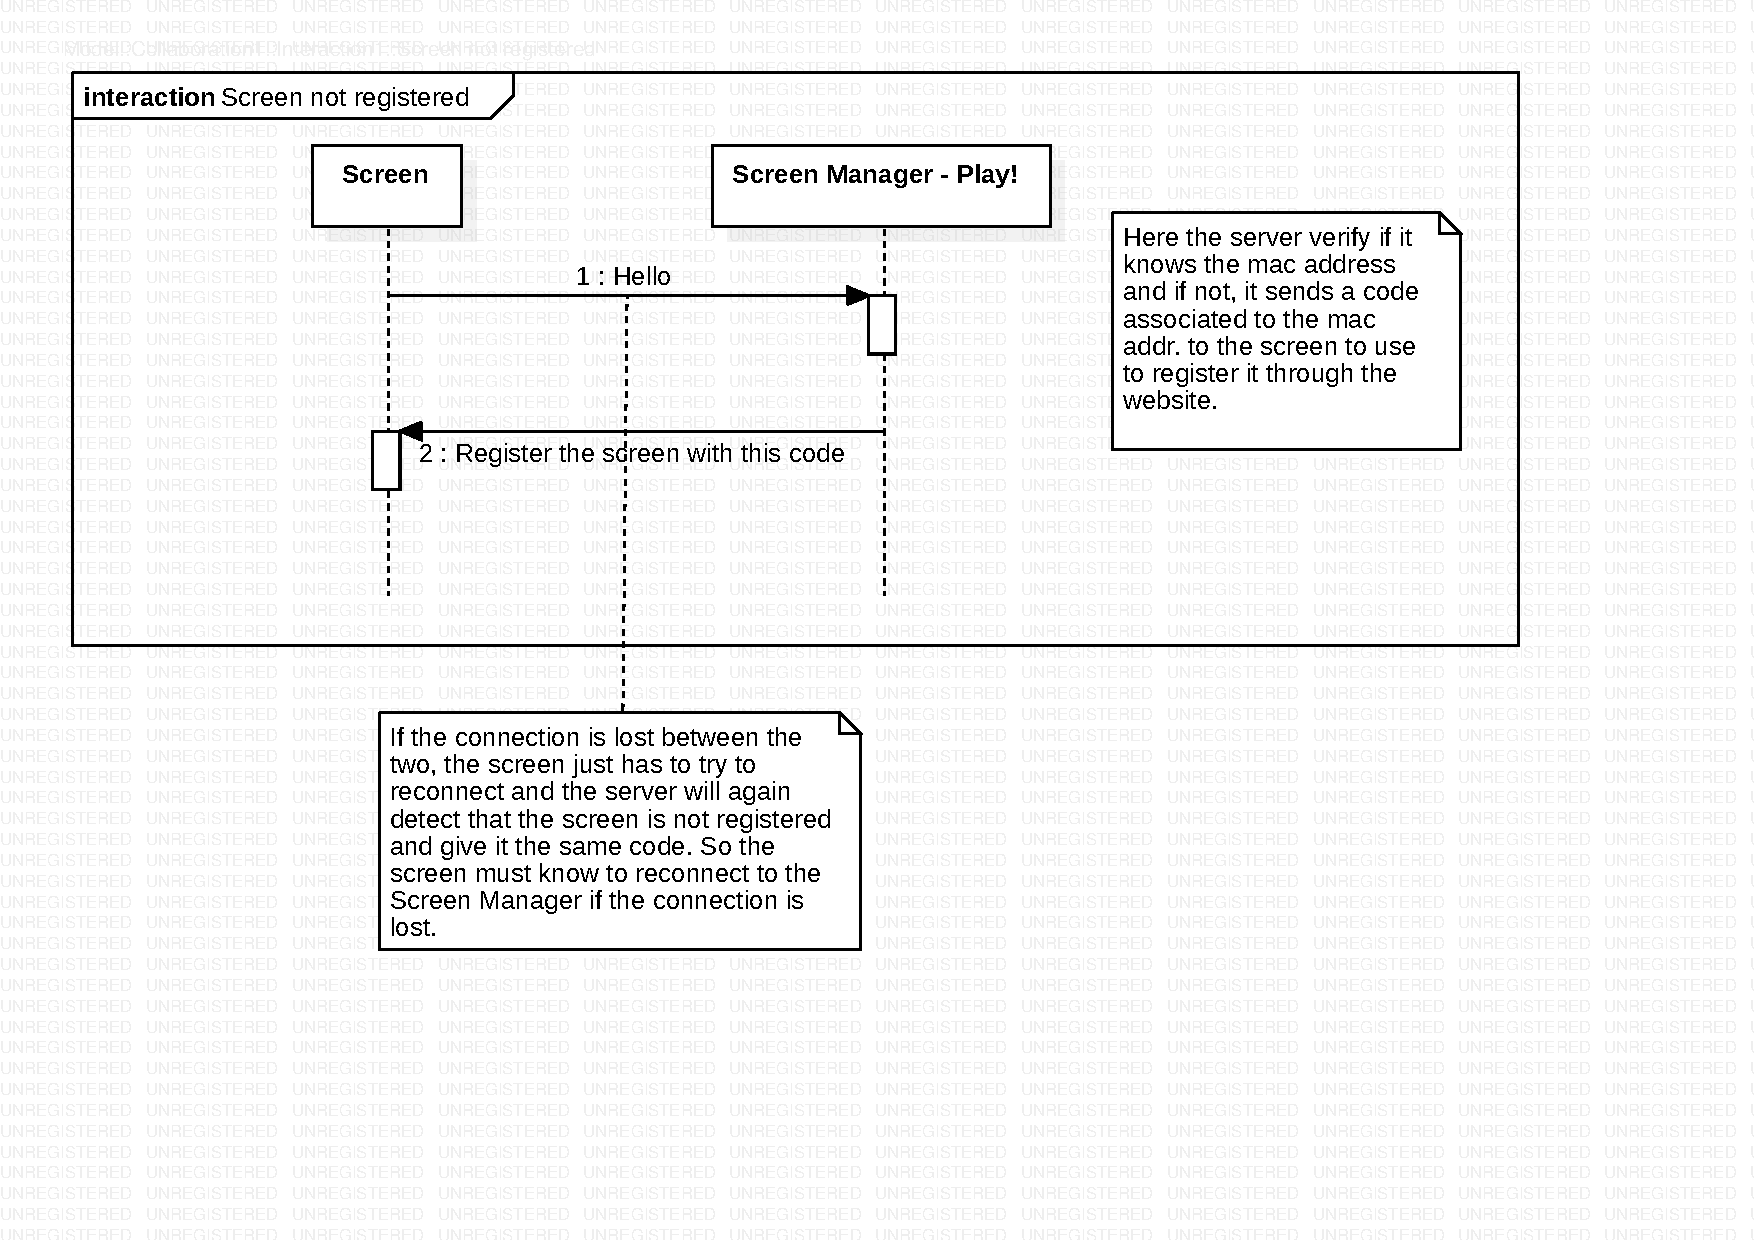
\includegraphics[page={1}, scale=0.5]{protocol_v2}
			\caption{Ecran inconnu}
		\end{figure}
	
	Le fait que l'écran perde sa connexion Internet pendant cet échange ne devrait poser aucun problème car le code sera simplement ré-envoyé à l'écran lors de sa prochaine connexion (en effet l'adresse MAC sera toujours inconnue du serveur). \newpage
	
\subsection{Ecran connu du serveur}
	La figure suivante décris le cas idéal, où l'écran est connu par le serveur et il n'y a pas de perte de connexion.
	\begin{figure}[h!]
		\centering
		\includegraphics[page={3}, scale=0.5]{protocol_v2}
		\caption{Ecran connu}
	\end{figure}			
	L'adresse MAC de l'écran est cette fois connue par le serveur, donc il marque l'écran comme actif (logged in) et vérifie si l'écran est associé avec un RunningSchedule. Si c'est le cas, il ajoute son adresse MAC dans la liste des écrans concernés par ce Schedule et le redirige vers le endpoint d'envoi d'Events. Dans le cas contraire, l'écran affiche simplement un message générique (p.ex. "Ecran non-assigné..."). \newpage
	
\subsection{Ecran connu - erreurs de connexion}
	Ici sont listées les actions effectuées par le serveur ou le client en cas d'erreurs lors la phase d'authentification.
	\begin{figure}[h!]
		\centering
		\includegraphics[page={2}, scale=0.5]{protocol_v2}
		\caption{Ecran connu - erreurs}
	\end{figure}
	
			
	Comme précédemment, le fait qu'un écran perde sa connexion au serveur lorsqu'il essaie de s'authentifier ne devrait pas poser de problèmes, car il lui suffit de ré-essayer. \newline
	Par contre, si l'écran perd sa connexion une fois qu'il s'est identifié auprès du serveur, il faudra le retirer de la liste des écrans concernés par son RunningSchedule jusqu'à ce qu'il se re-connecte. \newpage

	
\section{Schéma de base de donnée}
Une des directives principales du projet était la représentation en tout temps de l'état actuel du programme en base de données. Le schéma a donc été pensé pour répondre à cette demande. Les limitations voulues pour les différents rôles des utilisateurs et pour les services de la HEIG (COM, Secrétariat, Baleinev, etc) sont toutes représentées en BD, comme par exemple un PhysicalScreen est relié à un site (ce qui limite les flux qu'il peut afficher) et il est également relié à une ou plusieurs Teams (autorise uniquement les membres de cette Team à interagir avec cet écran).
\newline TODO : explications du schéma une fois celui-ci définitif (ou presque).

	\begin{figure}[h]
		\centering
		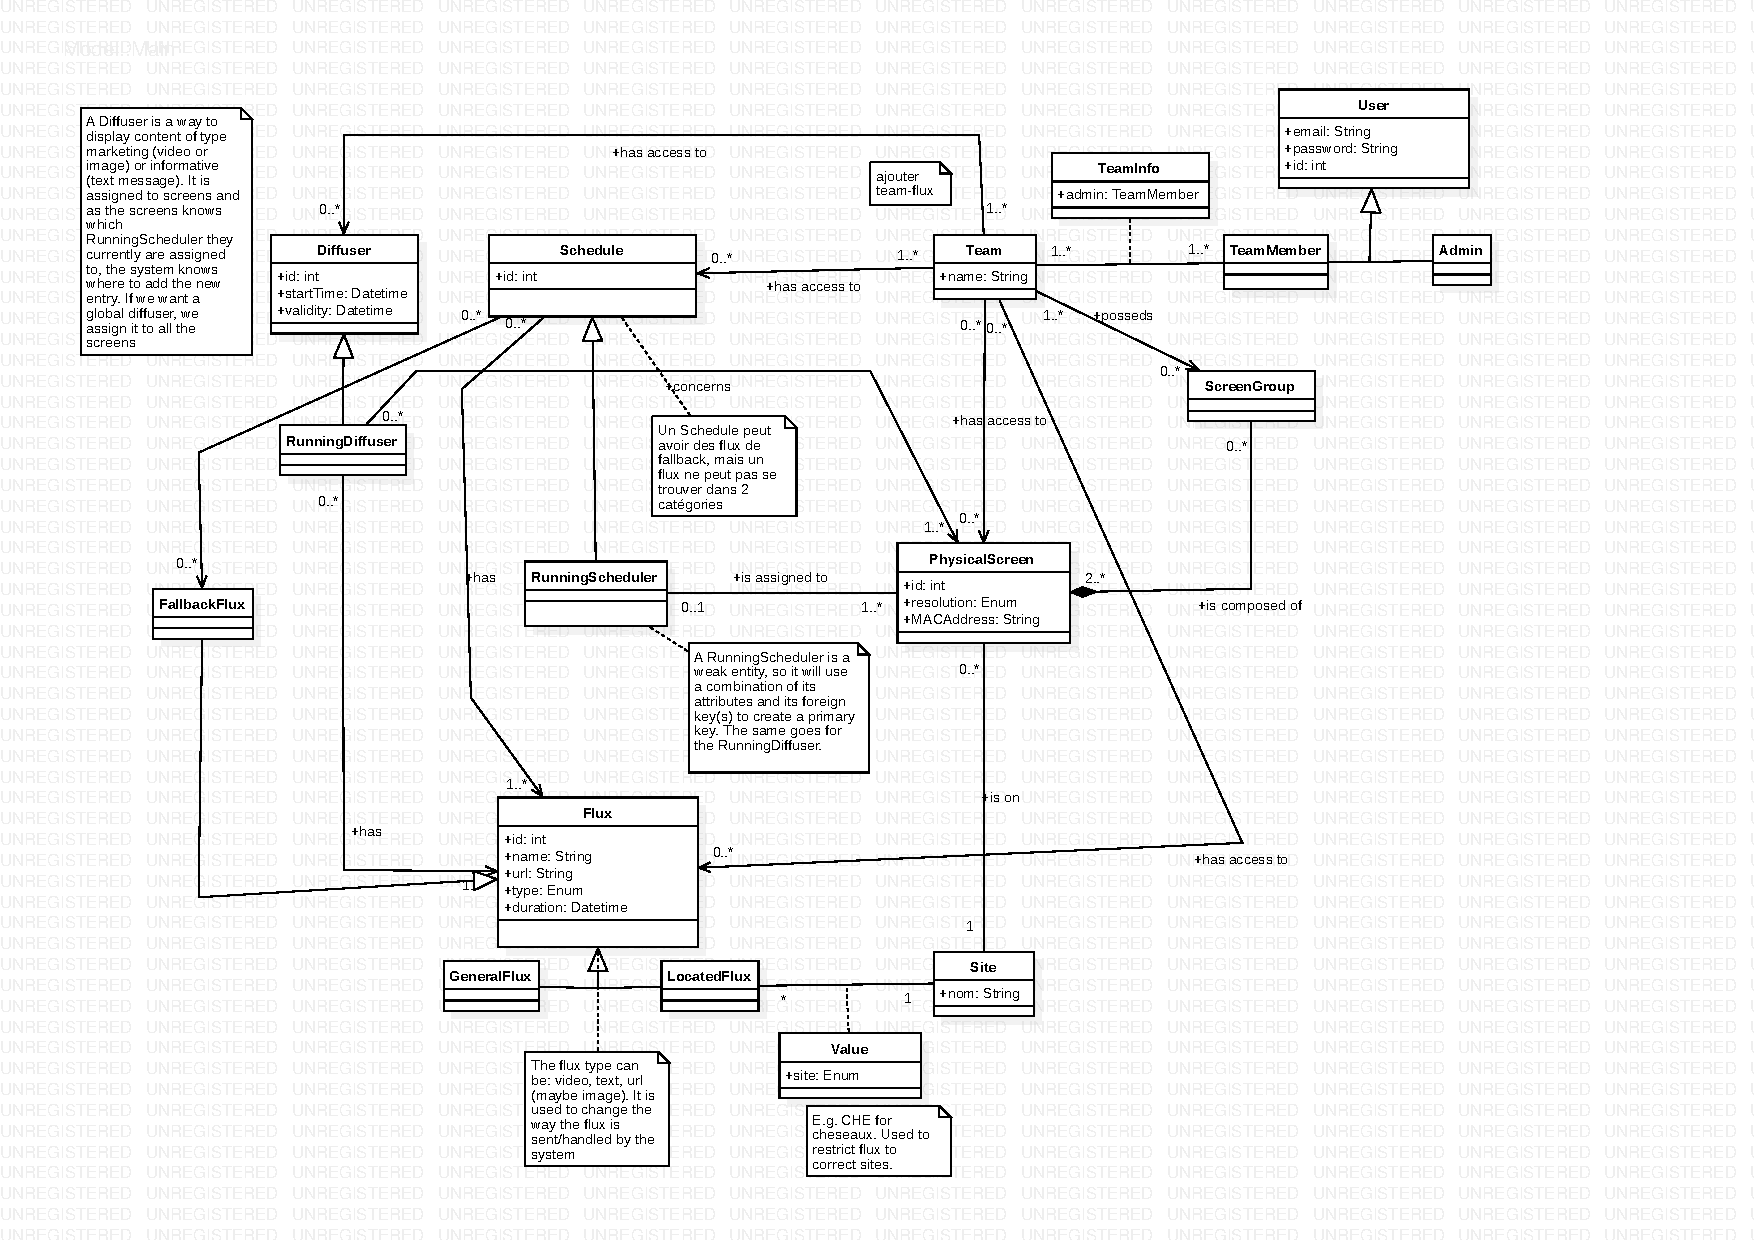
\includegraphics[scale=0.5]{db_schema}
		\caption{Schéma de base de données}
	\end{figure}
	
	
\newpage	

	
\section{Cas d'utilisation}
Les cas d'utilisation suivants sont regroupé par catégorie d'utilisateurs. Il y en a trois : les administrateurs, les chefs d'équipe (TeamAdmin) et les simples membres d'une équipe (TeamMember). Les admins ne sont associés à aucun écrans tandis que les deux autres sont restreints à certains écrans.
Toute action possible pour une catégorie l'est également pour celles en dessus. 

	\subsection{Administrateur:}
	L'admin peut effectuer toutes les actions et est le seul à pouvoir ajouter ou supprimer des écrans ou des utilisateurs au système. L'écran est allumé et connecté dans tous les cas suivants. \newline
		\begin{itemize}
		\item \textbf{Scénario 1:} Ajout d'un écran\newline
		\textbf{Déroulement:} L'admin rentre l'URL d'authentification des écrans dans le navigateur en spécifiant l'adresse MAC de l'écran comme paramètre de requête. Le serveur ne reconnait pas l'adresse MAC envoyée et renvoie donc un code servant à enregistrer l'écran dans le système. L'admin passe donc par le site pour ajouter l'écran en spécifiant entre autres son adresse MAC, son emplacement et le code fourni précédemment.\newline
		\textbf{Résultat:} L'écran sera maintenant reconnu par le serveur et correctement redirigé à la prochaine tentative.\newline
		\textbf{Erreurs potentielles:} Si la connexion est perdue entre l'écran et le backend à n'importe quel moment du scénario, les mêmes opérations seront effectuées à la re-connexion de l'écran (envoi du code). \newline
		
		\item \textbf{Scénario 2:} Mise à jour des infos d'un écran\newline
		\textbf{Pré-requis:} l'écran est déjà connu par le système.\newline
		\textbf{Déroulement:} L'admin se connecte au site et utilise l'interface fournie pour mettre à jour les infos souhaitées (nécessite potentiellement que l'écran ne soit pas actif).\newline
		\textbf{Résultat:} L'admin est informé du succès (ou de l'échec) de l'opération.\newline
		
		\item \textbf{Scénario 3:} Suppression d'un écran\newline
		\textbf{Pré-requis:} l'écran est déjà connu par le système.\newline
		\textbf{Déroulement:} L'admin se connecte au site et supprime l'écran du système en utilisant l'interface.\newline
		\textbf{Résultat:} L'admin est informé du succès (ou de l'échec) de l'opération et l'adresse MAC de l'écran est supprimée du système.\newline

		\item \textbf{Scénario 4:} Ajout d'un utilisateur\newline
		\textbf{Déroulement:} L'admin se connecte au site et ajoute l'utilisateur en utilisant l'interface fournie. Lors de l'ajout, il spécifie les écrans auxquels l'utilisateur pourra assigner des Schedules.\newline
		\textbf{Résultat:} L'admin est informé du succès (ou de l'échec) de l'opération et l'utilisateur est ajouté à la base de donnée.\newline

		\item \textbf{Scénario 5:} Modération: désactivation de Schedule\newline
		\textbf{Pré-requis:} Le Schedule est activé.\newline
		\textbf{Déroulement:} L'admin se connecte au site et va sur la page des Schedules. Dans la liste des actifs, il sélectionne celui qu'il veut désactiver et confirme son choix.\newline
		\textbf{Résultat:} L'admin est informé du succès (ou de l'échec) de l'opération et le Schedule est désactivé.\newline
		
		\item \textbf{Scénario 6:} Création d'une Team\newline
		\textbf{Déroulement:} L'admin se connecte au site et va sur la page des Teams. Il utilise l'interface fournie pour créer une nouvelle Team. Il doit spécifier à la création le nom de la Team et les écrans accessibles par ses membres. \newline
		\textbf{Résultat:} L'admin est informé du succès (ou de l'échec) de l'opération et la Team est créée et ajoutée en BD.\newline
		\textbf{Erreurs potentielles:} 
			\begin{itemize}
				\item Si le nom choisi pour la Team existe déjà, une erreur sera lancée et l'admin devra en choisir un autre. 
			\end{itemize}
			
		\item \textbf{Scénario 7:} Modification d'une Team\newline
		\textbf{Pré-requis:} La Team existe.\newline
		\textbf{Déroulement:} L'admin se connecte au site et va sur la page des Teams. Il utilise la même interface que pour la création pour mettre à jour les infos souhaitées (nom, membres, admin).\newline
		\textbf{Résultat:} L'admin est informé du succès (ou de l'échec) de l'opération et la Team est modifiée.\newline
		\textbf{Erreurs potentielles:} 
			\begin{itemize}
				\item Si le nom choisi pour la Team existe déjà, une erreur sera lancée et l'admin devra en choisir un autre. \newline
			\end{itemize}
		
		\item \textbf{Scénario 8:} Suppression d'une Team\newline
		\textbf{Pré-requis:} La Team existe.\newline
		\textbf{Déroulement:} L'admin se connecte au site et va sur la page des Teams. Il sélectionne dans la liste celle qu'il souhaite supprimer et utilise l'interface fournie pour le faire. \newline
		\textbf{Résultat:} L'admin est informé du succès (ou de l'échec) de l'opération et la Team est supprimée. Les entités associés avec cette équipe sont également supprimées (Schedules et Diffuser). \newline

					
		\end{itemize}
		\newpage
	 
	\subsection{TeamAdmin:} 
	Un TeamAdmin ne peut ajouter d'écrans mais a la permission d'activer Schedules et Diffusers. \newline
		\begin{itemize}	
			\item \textbf{Scénario 1:} Activation d'un Schedule\newline
			\textbf{Pré-requis:} Le Schedule existe et les écrans choisis ne sont pas déjà assignés à un autre Schedule.\newline
			\textbf{Déroulement:} Le TeamAdmin se connecte au site et va sur la page des Schedules. Il choisit dans la liste affichée celui qu'il veut activer et utilise l'interface pour assigner des écrans ou groupes d'écrans à ce Schedule. Il peut ensuite activer son Schedule. \newline
			\textbf{Résultat:} Le TeamAdmin est informé du succès (ou de l'échec) de l'opération.\newline
			\textbf{Erreurs potentielles:} 
			\begin{itemize}
				\item Si le Schedule contient un flux restreint à un site et que l'on l'assigne à un écran sur un autre site, le système nous empêchera de le faire. Par contre, assigner un groupe d'écran avec un sous-ensemble de ce groupe d'un site différent sera possible (un flux de backup sera diffusé sur cet écran à la place).
				\item Si, parmi les écrans choisis, un ou plusieurs sont déjà assignés à un Schedule, le TeamAdmin en est prévenu et doit changer sa sélection. \newline
			\end{itemize}			
		
		\item \textbf{Scénario 2:} Activation d'un Diffuser\newline
			\textbf{Pré-requis:} Le Diffuser existe et les écrans choisis sont assignés à un Schedule.\newline
			\textbf{Déroulement:} Le TeamAdmin se connecte au site et va sur la page des Diffusers. Il choisit dans la liste affichée celui qu'il veut activer et utilise l'interface pour assigner des écrans ou groupes d'écrans à ce Diffuser. Il peut ensuite l'activer. \newline
			\textbf{Résultat:} Le TeamAdmin est informé du succès (ou de l'échec) de l'opération.\newline
			\textbf{Erreurs potentielles:} 
			\begin{itemize}
				\item L'heure de début prévue pour le flux du Diffuser est identique (ou à peine après) à l'heure de début d'un flux du Schedule. Il y a plusieurs manières de traiter ce cas: checker la durée du nouveau flux et reprendre l'exécution de l'ancien une fois fini, repousser un des deux flux (pas top je pense).\newline
			\end{itemize}			
			   
		\item \textbf{Scénario 3:} Création de groupe d'écrans\newline
			\textbf{Déroulement:} Le TeamAdmin se connecte au site et va sur la page des écrans. Il choisit les écrans (au moins 2) dans la liste pour son groupe et confirme son choix. (Les écrans peuvent appartenir à plusieurs groupes) \newline
			\textbf{Résultat:} Le TeamAdmin est informé du succès (ou de l'échec) de l'opération et le groupe est créé en BD.\newline	
			\textbf{Erreurs potentielles:} 
			\begin{itemize}
				\item Moins de 2 écrans sont choisis, le TeamAdmin est informé et doit choisir plus d'écrans.\newline
			\end{itemize}
			
		\item \textbf{Scénario 4:} Modification de groupe d'écrans\newline
			\textbf{Pré-requis:} Le groupe existe.\newline
			\textbf{Déroulement:} Le TeamAdmin se connecte au site et va sur la page des écrans/groupes. Il choisit dans la liste des groupes celui ou ceux qu'il désire modifier et utilise pour ce faire la même interface que pour la création de groupe. \newline
			\textbf{Résultat:} Le TeamAdmin est informé du succès (ou de l'échec) de l'opération et le groupe est modifié en BD.\newline	
			\textbf{Erreurs potentielles:} 
			\begin{itemize}
				\item Si le groupe est actuellement assigné à un RunningSchedule, la modification est empêchée et le TeamAdmin en est informé.
				\item Si le groupe modifié contient moins de deux écrans, la modification est empêchée et le TeamAdmin en est informé.\newline
			\end{itemize}
			
		\item \textbf{Scénario 5:} Suppression de groupe d'écrans\newline
			\textbf{Pré-requis:} Le groupe existe.\newline
			\textbf{Déroulement:} Le TeamAdmin se connecte au site et va sur la page des écrans/groupes. Il choisit dans la liste des groupes celui ou ceux qu'il désire supprimer et utilise l'interface fournie pour le faire. \newline
			\textbf{Résultat:} Le TeamAdmin est informé du succès (ou de l'échec) de l'opération et le groupe est supprimé en BD.\newline	
			\textbf{Erreurs potentielles:} 
			\begin{itemize}
				\item Si le groupe est actuellement assigné à un RunningSchedule, la suppression est empêchée et le TeamAdmin en est informé.\newline
			\end{itemize}
		
		\end{itemize}
		
		
	\subsection{TeamMember:} 
	Un TeamMember est assigné à une Team, qui elle à accès à des écrans, Schedules et Diffusers. Il peut créer et modifier des Schedules et Diffuser non-actifs mais ne peut pas les activer. Comme tous les autres types d'utilisateurs, il peut créer des flux. \newline
		\begin{itemize}
			\item \textbf{Scénario 1:} Création d'un flux\newline
			\textbf{Déroulement:} Le TeamMember se connecte au site et va sur la page des flux. Il entre les paramètres de son flux (à définir) \newline
			\textbf{Résultat:} Le TeamMember est informé du succès (ou de l'échec) de l'opération et le flux est ajouté à la liste des flux disponibles.\newline
			
			\item \textbf{Scénario 2:} Modification d'un flux\newline
			\textbf{Pré-requis:} Le flux existe.\newline
			\textbf{Déroulement:} Le TeamMember se connecte au site et va sur la page des flux. Il choisit le flux à modifier dans la liste et utilise la même interface que pour la création pour la mise à jour. \newline
			\textbf{Résultat:} Le TeamMember est informé du succès (ou de l'échec) de l'opération.\newline
			
			\item \textbf{Scénario 3:} Suppression d'un flux\newline
			\textbf{Pré-requis:} Le flux existe.\newline
			\textbf{Déroulement:} Le TeamMember se connecte au site et va sur la page des flux. Il choisit le flux à supprimer et confirme son choix.\newline
			\textbf{Résultat:} Le TeamMember est informé du succès (ou de l'échec) de l'opération et le flux est retiré de la liste des flux disponibles.\newline
			
			\item \textbf{Scénario 4:} Création d'un Schedule\newline
			\textbf{Pré-requis:} Des flux ont préalablement été créés.\newline
			\textbf{Déroulement:} Le TeamMember se connecte au site et va sur la page de création de Schedules. Il choisit les heures de début des flux en associant le flux voulu. Il peut encore spécifier le nom du Schedule ou un commentaire sur son utilité. Il confirme son choix. \newline
			\textbf{Résultat:} Le TeamMember est informé du succès (ou de l'échec) de l'opération et le Schedule est ajouté à la liste des Schedules disponibles.\newline
			\textbf{Erreurs potentielles:} Les heures de début de flux ne sont pas cohérentes (confirmation alors impossible). \newline
			
			\item \textbf{Scénario 5:} Modification d'un Schedule \newline
			\textbf{Pré-requis:} Le Schedule existe.\newline
			\textbf{Déroulement:} Le TeamMember se connecte au site et va sur la page des Schedules. Il choisit le Schedule à modifier dans la liste et utilise la même interface que pour la création pour la mise à jour. \newline
			\textbf{Résultat:} Le TeamMember est informé du succès (ou de l'échec) de l'opération.\newline
			\textbf{Erreurs potentielles:} Les heures de début des nouveaux flux ne sont pas cohérentes (confirmation alors impossible). \newline
			
			\item \textbf{Scénario 6:} Création d'un Diffuser\newline
			\textbf{Pré-requis:} Des flux ont préalablement été créés.\newline
			\textbf{Déroulement:} Le TeamMember se connecte au site et va sur la page de création de Diffuser. Il choisit les heures de début du flux voulu et précise sa durée de validité (en jours?, semaines?). Il peut encore spécifier le nom du Diffuser ou un commentaire sur son utilité. Il confirme son choix. \newline
			\textbf{Résultat:} Le TeamMember est informé du succès (ou de l'échec) de l'opération et le Diffuser est ajouté à la liste des Diffusers disponibles.\newline
			\textbf{Erreurs potentielles:} Les heures de début de flux ne sont pas cohérentes (confirmation alors impossible). \newline
			
			\item \textbf{Scénario 7:} Modification d'un Diffuser \newline
			\textbf{Pré-requis:} Le Diffuser existe.\newline
			\textbf{Déroulement:} Le TeamMember se connecte au site et va sur la page des Diffuser. Il choisit le Diffuser à modifier dans la liste et utilise la même interface que pour la création pour la mise à jour. \newline
			\textbf{Résultat:} Le TeamMember est informé du succès (ou de l'échec) de l'opération.\newline
			\textbf{Erreurs potentielles:} Les heures de début des nouveaux flux ne sont pas cohérentes (confirmation alors impossible). \newline

		\end{itemize}
	
\section{Tests}

\subsection{Tests JUnit}

\subsection{Tests fonctionnels}

\section{Remarques personnelles et commentaires}


\end{document}
















